\subsection{Introduction}\label{sec:introduction}

The task of delivering Visual Semantic Navigation (VSN) capabilities to real robots in the real world is still a challenge.
To teach robots how to navigate in indoor environments, the VSN community has been using online reinforcement learning (RL) algorithms, which require querying environments to learn.
This is a problem because querying real environments is expensive and time-consuming, and querying simulated environments is not always a good proxy for real-world performance.
Offline RL~\cite{levine2020} can be a solution to these challenges by learning policies from a fixed dataset consisting in human demonstrations and their associated reward signals.
Therefore, in this work, we propose a novel approach to train VSN agents without ever querying an environment, by leveraging on the Offline RL paradigm.
We call this approach \textbf{Off}line Visual Semantic \textbf{Nav}igation (OffNav).

Technically, we have implemented Implicit Q-Learning (IQL)~\cite{kostrikov2022offline} offline RL algorithm using the decentralized distributed philosophy of DD-PPO~\cite{wijmans2020} to create DD-IQL, a decentralized distributed version of IQL\@.
Our DD-IQL is trained against a fixed dataset containing thousands of human navigation experiences~\cite{ramrakhya2023}.
As depicted in Figure~\ref{fig:abstract}, we propose the OffNav approach, capable of efficiently learning the navigation policy required by a VSN agent from human demonstrations.
Subsequently, these policies can be deployed across various scenarios, and if necessary, further refined through online RL for more specific tasks.

To demonstrate the capabilities of our implementation, we carried out a small analysis of its performance using different environments from HM3D dataset~\cite{Ramakrishnan2021HabitatMatterport3D}.
Preliminary results shows that our DD-IQL implementation is able to learn navigation policies effectively.
To the best of our knowledge, this is the first time that an offline RL algorithm is implemented for VSN\@ and large environments, predicting actions directly from raw input observations.

\begin{figure}
    \centering
    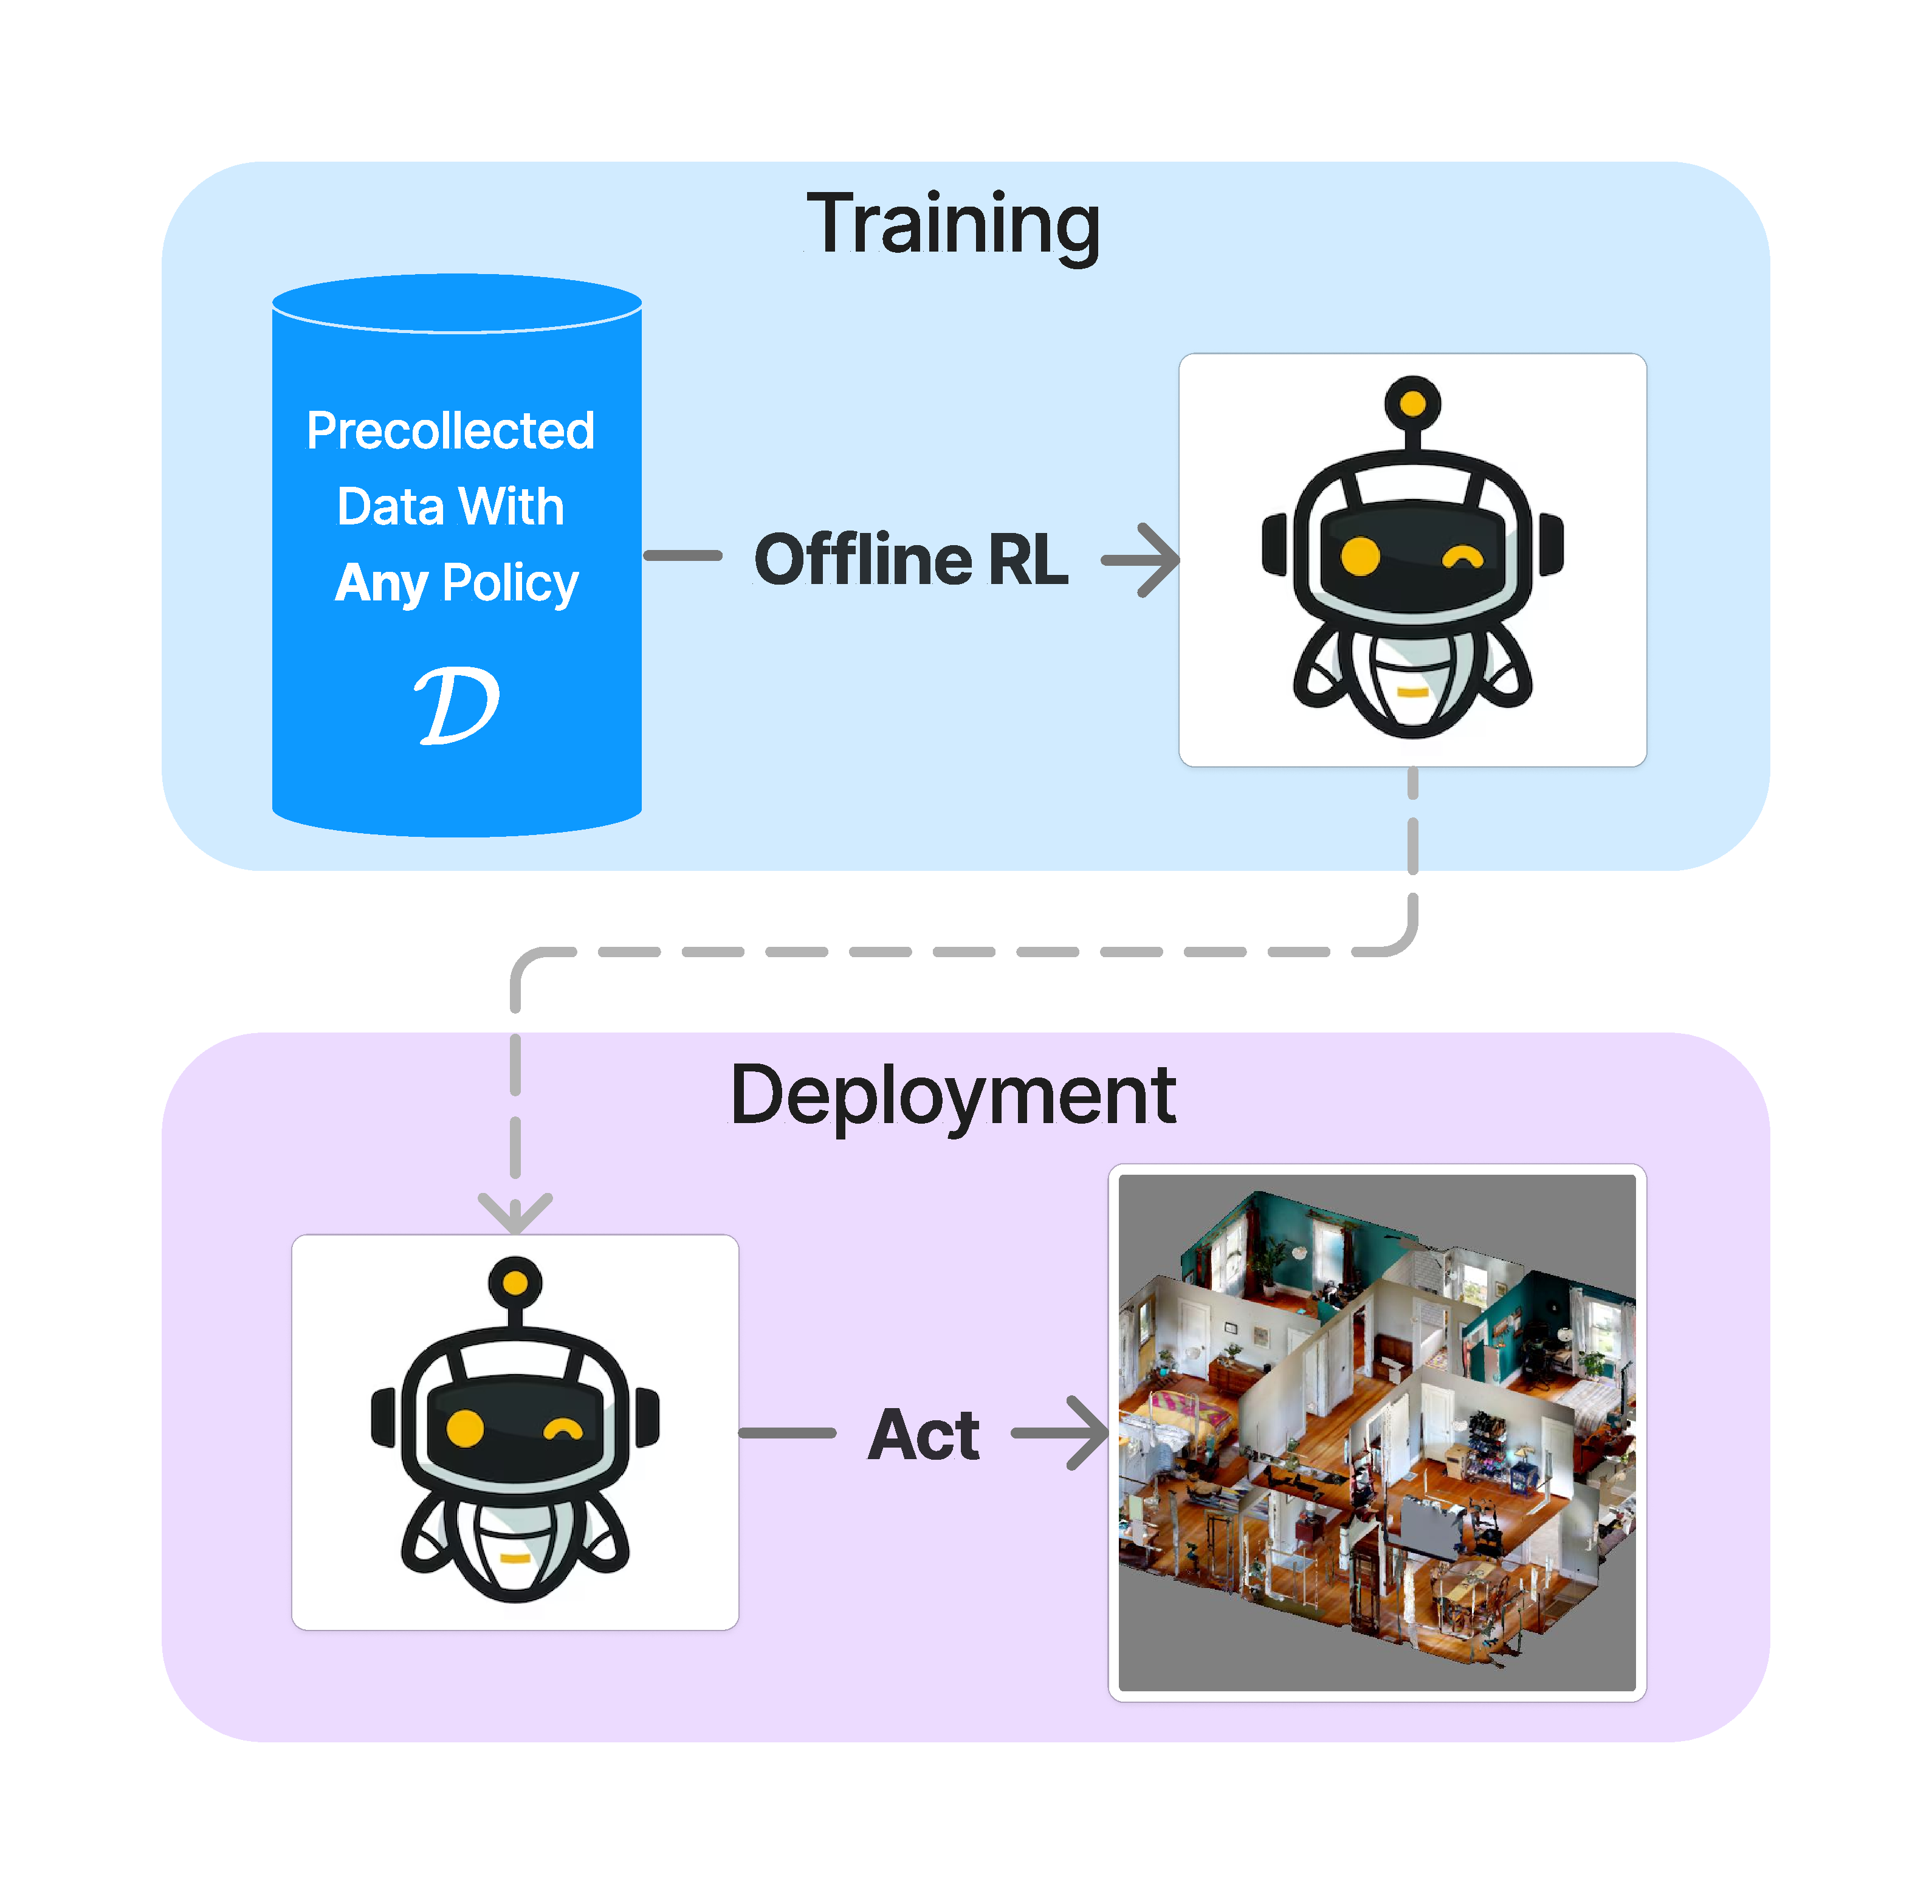
\includegraphics[width=.8\linewidth]{figures/offnav/graphical_abstract}
    \caption{
    By leveraging on the offline reinforcement learning paradigm, we can train agents from a fixed dataset of navigation experience, without querying any environment.
    This opens the possibility to create many navigation datasets from any navigation agent in any \textbf{real or simulated} environment, and then use them to train new agents for different scenarios without the need to ever query that environment.
    }
    \label{fig:abstract}
\end{figure}

%Current state-of-the-art models~\cite{ramrakhya2023} achieve 70,4\% SR on Habitat Simulator~\cite{szot2021} by using a two-phase training schedule.
%First, a


%% Maybe for experiments
%If the agent successfully reaches the object within a time limit, the episode is considered successful.
%In the other case, it is considered a failure.
%The performance of the navigation is measured by averaging the success over all the episodes present in an evaluation, and it receives the name of Success Rate (SR).
%%%%%%%%%%%%%%%%%%%%%%%%%%%

